\documentclass[11pt]{article}
\usepackage{amsmath,amssymb,color,hyperref,graphicx,pdfsync}
\usepackage{textcomp}
\usepackage{setspace}
\usepackage{fancyvrb}
\usepackage{svn}
\SVN $Date$
\SVN $Revision$
\SVN $Author$
\SVN $HeadURL$
\newcommand\revisioninfo{\centerline{\textcolor{blue}{Revision: \SVNRevision ; Last changed by \SVNAuthor\ on \SVNDate .}}}

\graphicspath{{Figures/}}

\textwidth 5.5 truein
\oddsidemargin .5 truein
\evensidemargin .5 truein
\topmargin -.5 truein
\textheight 8.5in

\definecolor{gray}{gray}{0.5}
\definecolor{green}{rgb}{0,0.5,0}

\def\class#1{\textcolor{green}{\bf #1}}
\def\todo#1{\textcolor{blue}{{\bf To do:} #1}}
\def\question#1{\textcolor{red}{\bf Question:} #1}

%\def\code#1{{\ttfamily #1}}
\def\class#1{\textcolor{green}{\ttfamily\small #1}} % \bfseries
\def\fn#1{{\ttfamily\small #1}} % \ttfamily
\def\virtualfn#1{{\ttfamily\small\slshape #1}} % \itshape

\begin{document}

\title{Manual for Immersed Boundary Projection Method (IBPM)}
\author{Clancy Rowley}
\date{\revisioninfo}
\maketitle

\section{Overview}
The code described in this manual uses an immersed boundary method to solve the two-dimensional incompressible Navier-Stokes equations around complex geometries, using the projection method described in~\cite{TaiCol-06}.  In particular, this code implements the ``fast method'' described in Section 3.3 of~\cite{ColTai-07}, using the multi-domain approach for far-field boundary conditions, as described in section~4 of~\cite{ColTai-07}.

\subsection{How this manual is organized}
\label{ssub:how_this_manual_is_organized}

This package provides a command-line tool ({\tt ibpm}), as well as a library ({\tt libibpm.a}) that can be used for writing customized programs, such as post-processing utilities, or computational wrappers around the main solver.

Section~\ref{sec:install} describes how to compile the library and executables.  Section~\ref{sec:method} describes what the code does, giving the highlights of the numerical method.  Section~\ref{sec:commandline} describes the simplest way to use the code, via the command-line tool.  Section~\ref{sec:library} describes the high-level classes provided by the library, geared towards users of the library.  More detailed documentation of the library (e.g., for developers making additions to the library) can also be generated (see Section~\ref{sec:install} below).

\section{Installation}
\label{sec:install}
\subsection{System requirements}
To compile and run the code, you will need the following:
\begin{itemize}
	\item A C++ compiler
	\item The FFTW library, version~3, available free from \url{http://www.fftw.org/}
\end{itemize}
We assume you are building on a Unix-based system, such as Mac OS X or Linux, and have standard build tools such as GNU Make.

The package includes a suite of automated tests, and if you would like to run these, you will need the Google C++ Testing Framework, version 1.3.0, available free from \url{http://code.google.com/p/googletest/}.

Detailed documentation for the library can also be generated, in html and/or \LaTeX\ formats.  To generate the documentation you will need the Doxygen tool, available at \url{http://www.stack.nl/~dimitri/doxygen/}.

\subsection{Building the library and executables}
The default configuration is to compile the code with the GCC compiler, with the FFTW library in a default location known to the compiler (e.g. {\tt /usr/local/lib}).  If this is acceptable, then to build the library and executables, all you need to do is type {\tt make} from the root {\tt ibpm} directory.  The library and command-line tools will be generated in the {\tt build} directory.

In order to customize the build process for your system, make a copy of the file {\tt config/make.inc.gcc} and modify it as needed (this is included in the main Makefiles, and the format is pretty self-explanatory).  The new configuration file should be named {\tt config/make.inc}.  Then type {\tt make} from the root {\tt ibpm} directory, as before.

To build and run the automated tests, type {\tt make test}.

\subsection{Building the documentation}
To build the detailed documentation, type {\tt make doc}.  The default configuration is to generate both html and \LaTeX\ documentation, but this can be changed by modifying {\tt doc/Doxyfile}, for instance by changing the line {\tt GENERATE\_LATEX = YES} to {\tt GENERATE\_LATEX = NO}.  Once the documentation has been built, the html documentation (usually the most useful) can be found in {\tt doc/html/index.html}, and the \LaTeX\ documentation can be found in {\tt doc/latex/refman.tex}.

\section{What the code does}
\label{sec:method}
For details of the numerical method this code solves, see~\cite{ColTai-07}.  Here, we give only a brief overview.

\paragraph{Immersed boundary method}
The Navier-Stokes equations are solved in two dimensions, using a streamfunction-vorticity formulation, and a finite-volume method.  Thus, fluxes are defined on cell edges, and the scalar vorticity and streamfunction are defined at cell nodes.  Pressure is not used in this formulation.

Let $q$ denote the (vector-valued) velocity flux, $\psi$ the streamfunction, and $\omega$ the vorticity.  The no-slip boundary condition at the surface of an object is imposed by delta-function forces at the boundary locations, and $f$ is a vector of these force values.  The equations to be solved are given as (22) in~\cite{ColTai-07}:
\begin{align}
	\frac{d\omega}{dt} + C^TE^T\tilde f &= \nu L\omega + C^T(q\times\omega),
		\qquad \omega\big|_\partial = bc_\omega
		\label{eq:navier_stokes}\\
	L\psi &= -\omega,\qquad \psi\big|_\partial = bc_\psi
		\label{eq:poisson}\\
	EC\psi &= u_B.
		\label{eq:no_slip}
\end{align}
The first equation is the momentum equation, the second is a Poisson equation for the streamfunction, and the third equation is a constraint representing the no-slip condition, so that velocities at the boundary points match prescribed velocities~$u_B$. The discrete operators in the above equation are described in the table below, where $\nu=1/Re$ is one over the Reynolds number.  (Note that in~\cite{ColTai-07}, $\gamma$ denotes the circulation about one cell, while in this code we work with vorticity~$\omega$.  The two are related by $\gamma = \delta^2\omega$, where $\delta$ is the grid spacing.)
\begin{center}
\begin{tabular}{ccp{3.7in}}
Operator & Maps & Definition\\
$C$ 	& $\psi\mapsto q$ & curl of a scalar\\
$C^T$ 	& $q\mapsto \omega$ & curl of a vector in 2d\\
$S$ 	& $\omega\mapsto\hat\omega$ & discrete sin transform\\
$L=-C^TC$	& $\omega\mapsto\omega$ & Laplacian, analogous to $\triangle u = \nabla(\nabla\cdot u) - \nabla\times\nabla\times u$\\
$\Lambda$	& $\hat\omega\mapsto\hat\omega$ & eigenvalues of Laplacian\\
$E$ 	& $q\mapsto u_B$ & restriction of fluxes everywhere to velocities at boundary\\
$E^T$	& $f\mapsto q$ & regularization of forces at boundary points to fluxes everywhere\\
$D$		& $q\mapsto \varphi$ & divergence of a vector field
\end{tabular}
\end{center}
Here, $u_B$ is a vector of velocities at boundary points.  An important aspect of the method is that the curl operator~$C$ is chosen such that its range is in the nullspace of a discrete divergence operator~$D$, such that $DC=0$, and the continuity equation is satisfied for any streamfunction~$\psi$.  The discrete Laplacian $L$ is diagonalized by the discrete sin transform~$S$, and its eigenvalues are known analytically, so the Poisson equation~(\ref{eq:poisson}) can be solved efficiently.
To retrieve the fluxes $q$ from the streamfunction~$\psi$, we need to add in a (prescribed) potential flow solution~$q_\text{pot}$, so we have
\begin{equation}
	q = C\psi + q_\text{pot}.
\label{eq:compute_q}
\end{equation}
We consider farfield boundary conditions, for which $bc_\omega$ in~(\ref{eq:navier_stokes}) and~$bc_\psi$ in~(\ref{eq:poisson}) are both zero.

\paragraph{Time discretization}
Equation~(\ref{eq:navier_stokes}--\ref{eq:no_slip}) are stepped forward in time using a projection method, as follows.  For instance, discretizing the linear terms of (\ref{eq:navier_stokes}) using Crank-Nicolson (trapezoidal rule), and the nonlinear terms using explicit Euler, one obtains
\begin{align}
	\left(1-\frac{\nu\Delta t}{2}L\right)\omega^{n+1} + \Delta t C^TE^Tf &= \left(1 + \frac{\nu\Delta t}{2}L\right)\omega^n + \Delta t C^T (q^n\times\omega^n)  \label{eq:timestepper}\\
	-ECL^{-1}\omega^{n+1} &= u_B^{n+1}
\end{align}
These equations are of the form
\begin{equation}
	\begin{bmatrix}
		\mathcal{A} & \mathcal{B}\\\mathcal{C} & 0
	\end{bmatrix}
	\begin{bmatrix}
		\omega^{n+1}\\ f
	\end{bmatrix}
	=
	\begin{bmatrix}
		a\\b
	\end{bmatrix}
\label{eq:constrained}
\end{equation}
where
\begin{align}
	\mathcal{A} &= 1 - \frac{\nu\Delta t}{2}L\\
	\mathcal{B} &= \Delta t C^TE^T\\
	\mathcal{C} &= -ECL^{-1}\\
	a &= \left(1+\frac{\nu\Delta t}{2}L\right)\omega^n + \Delta t C^T(q^n\times\omega^n)\\
	b &= u_B.
\end{align}



\paragraph{Projection method}
We solve the constrained equation~(\ref{eq:constrained}) using the following algorithm:
\begin{equation}
\begin{aligned}
	\mathcal{A}\omega^* &= a,\qquad \omega^*\big|_\partial\\
	\mathcal{CA}^{-1}\mathcal{B}f &= \mathcal{C}\omega^* - b\\
	\omega^{n+1} &= \omega^* - \mathcal{A}^{-1}\mathcal{B}f
\end{aligned}
\label{eq:projection_alg}
\end{equation}
Since the matrix $\mathcal{A}$ is easily invertible using a sin transform, one may solve the first equation easily (applying boundary conditions on~$\omega^*$).  The second equation is rather small ($\text{\#forces} \times \text{\#forces}$), and furthermore the matrix $\mathcal{M}=\mathcal{C}\mathcal{A}^{-1}\mathcal{B}$ is symmetric, since $\mathcal{A}$ and $L$ have the same eigenvectors.  When the boundary conditions are fixed (stationary bodies), then the matrix~$\mathcal{M}$ is constant in time, and so may be LU decomposed (e.g. using a Cholesky decomposition) once beforehand, and solved rapidly at each timestep.  When the boundary conditions vary in time, then $E$ changes at each step, and a direct solve is not as efficient as an iterative solve, such as a conjugate-gradient method (also for symmetric matrices).

In~\cite{ColTai-07}, the algorithm for the timestepper~(\ref{eq:timestepper}) is coupled with the algorithm (\ref{eq:projection_alg}) for solving equation~(\ref{eq:constrained}), but in the design of the present code, these two algorithms are decoupled, so that different timesteppers may be interchanged easily.

\subsection{Multi-domain method}
For large domains, it is not practical to use uniform grid spacing, so the method in~\cite{ColTai-07} uses a multi-domain approach in which several nested uniform grids are used.  The Poisson equations may still be solved efficiently in this case, also using a number of sin transforms, as outlined here.  In the code, the only place the methods in this section are used is in the elliptic solvers (Poisson or Helmholtz equations---i.e., inverting the operators $L$ and $\mathcal{A}$ from the previous section).

One defines a scalar field $u$ on a nested set of grids $u^1,\ldots,u^{N_g}$, where $u^1$ is the finest grid and $u^{N_g}$ is the coarsest.  One then defines a sequence of {\em coarsening} operators $P^k$ that move points from the full grid $u$ to an individual coarse grid~$u^k$, by suitably averaging.  These coarsening operators are defined recursively, by starting with the finest grid and averaging values to each coarser grid sequentially.

In order to solve the system
\begin{equation}
	Lu = f,\qquad u\big|_\partial = bc_u,
\end{equation}
one first computes a sequence of coarsified forcing terms $f^1,\ldots,f^{N_g}$, for instance with $f^{k} = P^{k}f$. Then one considers the Laplacian $L_1$ on the finest (uniform) grid, and solves a sequence of Poisson problems
\begin{equation}
\begin{aligned}
	L_1 u^{N_g} &= 2^{N_g-1} f^{N_g},& u^{N_g}\big|_\partial &= bc_u\\
	L_1 u^{N_g-1} &= 2^{N_g-2} f^{N_g-1},& u^{N_g-1}\big|_\partial &= bc(u^{N_g})\\
	&\;\vdots\\
	L_1 u^1 &= f^1,& u^1\big|_\partial &= bc(u^2)
\end{aligned}
\end{equation}
where the operators $bc(u^{k+1})$ return the values on grid $u^{k+1}$ that are on the boundary of the next finer grid~$k$.  The scaling terms $2^k$ on the right-hand side compensate for the different grid spacings on the different domains.  Since the single-grid Laplacian $L_1$ is easily inverted using a sin transform, the overall solution is efficient.

\section{Using the command-line tools}
\label{sec:commandline}

This distribution provides a command-line tool ({\tt ibpm}) for running the main solver, as well as a simple tool ({\tt checkgeom}) for checking the syntax of geometry files, and verifying whether they are suitable for a given grid.

\subsection{Overview of the main IBPM tool}
\label{sub:overview_of_the_main_ibpm_tool}

The command-line tool {\tt ibpm} reads in a geometry file and an initial flow field (or initializes a default flow field of potential flow around the body), and advances the flow forward in time, writing various output files.  Parameters are specified as command-line arguments, and for a complete list of options with brief descriptions, run {\tt ibpm -h}.  

\paragraph{Grid}
Parameters related to the grid are specified as follows:

\begin{center}
\begin{tabular}{lll}
Flag & Description & Default\\
\hline
\verb|-nx <int>|         & number of grid cells in $x$-direction & 200\\
\verb|-ny <int>|         & number of grid cells in $y$-direction & 200\\
\verb|-ngrid <int>|      & number of grid levels for multi-domain scheme & 1\\
\verb|-length <real>|    & length of finest domain in $x$-dir & 4\\
\verb|-xoffset <real>|   & $x$-coordinate of left edge of finest domain & $-2$ \\
\verb|-yoffset <real>|   & $y$-coordinate of bottom edge of finest domain & $-2$\\
\end{tabular}
\end{center}

The grid spacing is ${\tt length}/{\tt dx}$, and is always the same in $x$ and $y$ directions, so the height in the $y$-direction is the $x$-length times {\tt ny/nx}.  Note that the arguments {\tt nx} and {\tt ny} specify the number of {\em cells\/} in each direction, so the number of grid points, including boundary points, is $({\tt nx}+1) \times ({\tt ny}+1)$, as shown in Figure~\ref{fig:grid}.
\begin{figure}
\begin{center}
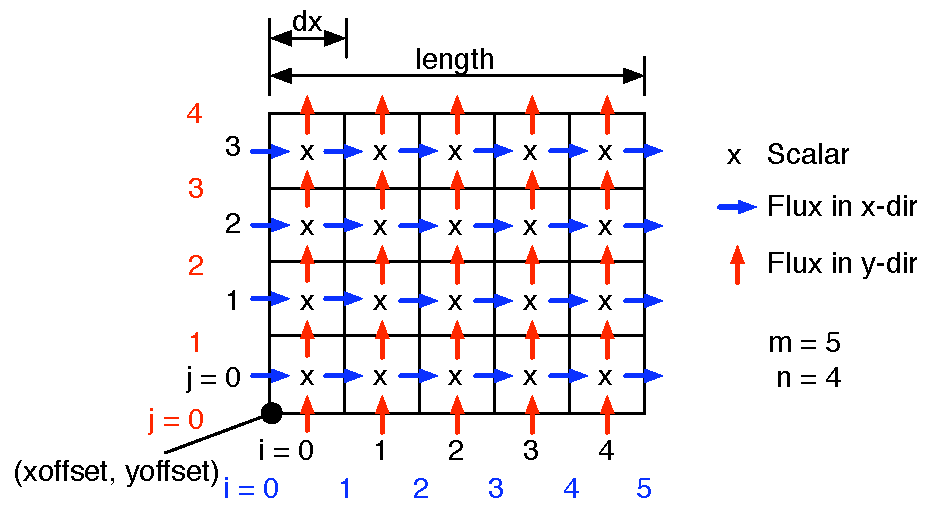
\includegraphics[width=\linewidth]{grid}
\caption{Layout of grid for the finite-volume method.  In output files, all variables are given at nodes ($\times$).}
\label{fig:grid}
\end{center}
\end{figure}

\paragraph{Geometry}
The geometry of the body is read from a file, and the filename is specified as follows:
\begin{center}
\begin{tabular}{lll}
Flag & Description & Default\\
\hline
\verb|-name <string>|    & name of the run & {\tt ibpm}\\
\verb|-geom <string>|    & filename for reading geometry & \verb|<name>.geom|
\end{tabular}
\end{center}
For instance, if {\tt -name foo} is specified, then the file {\tt foo.geom} is read.  If {\tt -name foo -geom bar.geom} is specified, then the file {\tt bar.geom} is read.

The format of the geometry file is discussed in Section~\ref{sub:defining_the_geometry}. The run name specified by {\tt -name} also determines the name of various output files (described below).

For instance, to run with a $200\times 300$ grid, for $x\in[-1,3]$ and $y\in [-3,3]$ on the finest grid, reading the geometry from the file {\tt myshape.geom}, execute
\begin{Verbatim}
ibpm -nx 200 -ny 300 -length 4 -xoffset -1 -yoffset -3 -geom myshape.geom
\end{Verbatim}


\paragraph{Solver}
Parameters related to the flow solver are specified as follows:

\begin{center}
\begin{tabular}{lp{2.3in}l}
Flag & Description & Default\\
\hline
\verb|-Re <real>|        & Reynolds number & 100\\
\verb|-dt <real>|        & timestep & 0.01\\
\verb|-model <string>|   & type of model (linear, nonlinear, adjoint, linearperiodic) & nonlinear\\
\verb|-baseflow <string>| & base flow for linear/adjoint model\\
\verb|-scheme <string>|   & timestepping scheme (euler, ab2, rk2, rk3) & rk2\\
\verb|-ic <string>|       & initial condition filename \\
\verb|-nsteps <int>|    & number of timesteps to compute & 250\\
\end{tabular}
\end{center}

The formulations of the linearized and adjoint Navier-Stokes equations are described in~\cite{AhuRow-08}, and if either of these options is used, then a filename must be given, for a restart file from which to load the base flow for the linearization (e.g., \verb|-model linear -baseflow steadystate.bin|).  To restart the solver from a given restart file, use the {\tt -ic} flag, as
\begin{Verbatim}
	ibpm -ic initial_condition.bin
\end{Verbatim}
Different timesteppers may be used, including explicit Euler ({\tt euler}), 2nd-order Adams-Bashforth ({\tt ab2}), and second- and third-order Runge-Kutta ({\tt rk2}, {\tt rk3}).

\paragraph{Output}
As the solution evolves in time, various output files can be written, and their output is specified as follows:

\begin{center}
\begin{tabular}{lll}
Flag & Description & Default\\
\hline
\verb|-outdir <string>| & directory for saving output & {\tt .}\\
\verb|-tecplot <int>|   & if $>0$, write a Tecplot file every $n$ timesteps & 100\\
\verb|-restart <int>|   & if $>0$, write a restart file every $n$ timesteps & 100\\
\verb|-force <int>|     & if $>0$, write forces every $n$ timesteps & 1\\
\end{tabular}
\end{center}
If the directory for output files does not exist, it is created, and all output files are written to this directory.  Forces are written to a single file, whose columns are:
\begin{Verbatim}
Timestep	Time	Lift coef	Drag coef
\end{Verbatim}
Tecplot files are ASCII files readable by the Tecplot visualization software, and restart files are binary files that can be used by {\tt ibpm} as initial conditions, base flows for linearization, etc.

The command-line options specified for the run are also written to a file \verb|<name>.cmd|.  Thus, any run can be repeated with
\begin{Verbatim}
. <outdir>/<name>.cmd
\end{Verbatim}

\paragraph{Periodic flows}
Additional options are needed when running simulations linearized about a periodic base flow (\verb|-model linearperiodic|):

\begin{center}
\begin{tabular}{lll}
Flag & Description & Default\\
\hline
\verb|-period <int>|    & period of periodic baseflow & 1\\
\verb|-periodstart <int>| & start time of periodic baseflow & 0\\
\verb|-pbaseflowname <string>| & name of periodic baseflow\\
\verb|-subbaseflow <0 or 1>| & Subtract baseflow from ic (1/0(true/false)) & 0\\
\verb|-numdigfilename <string>| & number of digits for time representation in filename & {\tt \%05d}
\end{tabular}
\end{center}

\subsection{Defining the geometry}
\label{sub:defining_the_geometry}
Here, we describe the format of the geometry file.  This file consists of a sequence of commands, all of the form
\begin{Verbatim}[gobble=4]
    <command> [argument 1] [argument 2] ... [argument n]
\end{Verbatim}
Whitespace is ignored, and only one command can be given on each line.  Comments can be included, using the comment character {\tt \#}.

A {\em geometry\/} consists of one or more {\em rigid bodies}.  A rigid body is a collection of points, specified by commands, which may be given in any order.  The following example illustrates the available commands:

\begin{Verbatim}[gobble=4]
    name Name of this object
    center x y  # location of the center of the object
    point x y   # add a point at this location
    point x y
    point x y
    line x1 y1 x2 y2 dx        # add a line, spacing dx
    line_n x1 y1 x2 y2 npts    # add a line with npts points
    circle xc yc radius dx     # add a circle, specifying spacing
    circle_n xc yc radius npts # add a circle, specifying num points
    raw naca0012.dat           # read a list of points from a file
    motion fixed x y theta     # assign a particular motion
\end{Verbatim}

The command {\tt line} constructs a line between points $(x_1,y_1)$ and $(x_2,y_2)$, with spacing {\tt dx} between points.  The command {\tt line\_n} constructs a similar line, but specifying the number of points instead of the spacing.  The {\tt circle} command behaves similarly, constructing a circle with the given center $(x_c,y_c)$ and radius, where the spacing between points on the circle is approximately {\tt dx}.

\paragraph{Note about spacing of boundary points}
The spacing between points on the boundary of a body should be smaller than the grid spacing, but not too small.  If the spacing is too coarse, fluid will ``leak'' through the boundary, and if the spacing is too fine, the solver may not converge.

\paragraph{Motion}
The points that make up a rigid body may be translated together by specifying a {\tt motion}.  The simplest motion is just translation and rotation, specified by
\begin{Verbatim}
motion fixed x y theta
\end{Verbatim}
which translates the body by $(x,y)$, and rotates about the center of the body by the angle {\tt theta} (expressed in radians).  This may be used, for instance, to incline an airfoil at a desired angle of attack.  The axis of rotation is defined using the {\tt center} command to specify its $x$- and $y$-coordinates.  One may also specify a pitch-plunge motion, as
\begin{Verbatim}
motion pitchplunge amp1 freq1 amp2 freq2
\end{Verbatim}
which specifies a translation and rotation given by
\begin{align*}
x(t) &= 0\\
y(t) &= A_2 \sin(2\pi f_2 t)\\
\theta(t) &= A_1 \sin(2\pi f_1 t)
\end{align*}
where $A_1,f_1$ are specified by {\tt amp1}, {\tt freq1}, etc.

\paragraph{Overall geometry}
The overall geometry is a collection of rigid bodies, for instance specified as follows:
\begin{Verbatim}[gobble=4]
    name My Geometry
    body Flat Plate
        line 0 0 1 0 0.1  # points on a line, spacing approximately 0.1
        center 0.25 0     # center at quarter chord
        motion fixed 0 0 0.3 # 0.3 radians angle of attack
    end
    body Large Circle
        circle 2 3 5 0.1 # Points on a circle
                         # default center is (2,3)
    end
    body Airfoil
        raw naca0012.in  # Read in a raw data file
    end
\end{Verbatim}

The {\tt name} command is optional, and whitespace is ignored.

\subsection{Tool for checking geometries}
\label{sub:tool_for_checking_geometries}
The program {\tt checkgeom} may be used to validate the syntax of geometry input files, and to plot the corresponding boundary points on a specified grid.  This is useful both to check that the geometry looks generally as expected before running a large simulation, but more importantly, it can be used to check for ``leaks'': as stated previously, if the boundary points are too coarsely spaced, relative to the underlying uniform grid, then the fluid can penetrate the boundary.

The options for {\tt checkgeom} are as follows:

\begin{center}
	\begin{tabular}{lll}
	  \verb|-h|                 & print a help message and exit \\
	  \verb|-nx <int>|          & number of gridpoints in $x$-direction & 200 \\
	  \verb|-ny <int>|          & number of gridpoints in $y$-direction & 200 \\
	  \verb|-ngrid <int>|       & number of grid levels for multi-domain scheme & 1 \\
	  \verb|-length <real>|     & length of finest domain in x-dir & 4 \\
	  \verb|-xoffset <real>|    & $x$-coordinate of left edge of finest domain & $-2$ \\
	  \verb|-yoffset <real>|    & $y$-coordinate of bottom edge of finest domain & $-2$ \\
	  \verb|-geom <string>|     & filename for reading geometry & ibpm.geom \\
	  \verb|-o <string>|       & filename for writing Tecplot file & [none]
	\end{tabular}
\end{center}

The default behavior is to read in a geometry file and exit normally if the file was successfully parsed.  In this case, the grid parameters are irrelevant.

If the name of an output file is given with the {\tt -o} flag, then as long as the file is successfully parsed, a Tecplot file is written, showing how the boundary points are regularized to the grid.  This Tecplot file can then be used to check for ``leaks.''

\section{Using the IBPM library}
\label{sec:library}

The algorithms used by the main {\tt ibpm} code are made available in a library that can be used by other codes, for instance to write wrapper routines around the main timestepper, or to perform post-processing tasks.  The library is written in an object-oriented style, with the various algorithms and data structures provided by different classes.  Here, we give an overview of the various classes and their roles.  For a detailed description of their interfaces, consult the Doxygen documentation, or the corresponding header files.

\begin{figure}
	\centering
		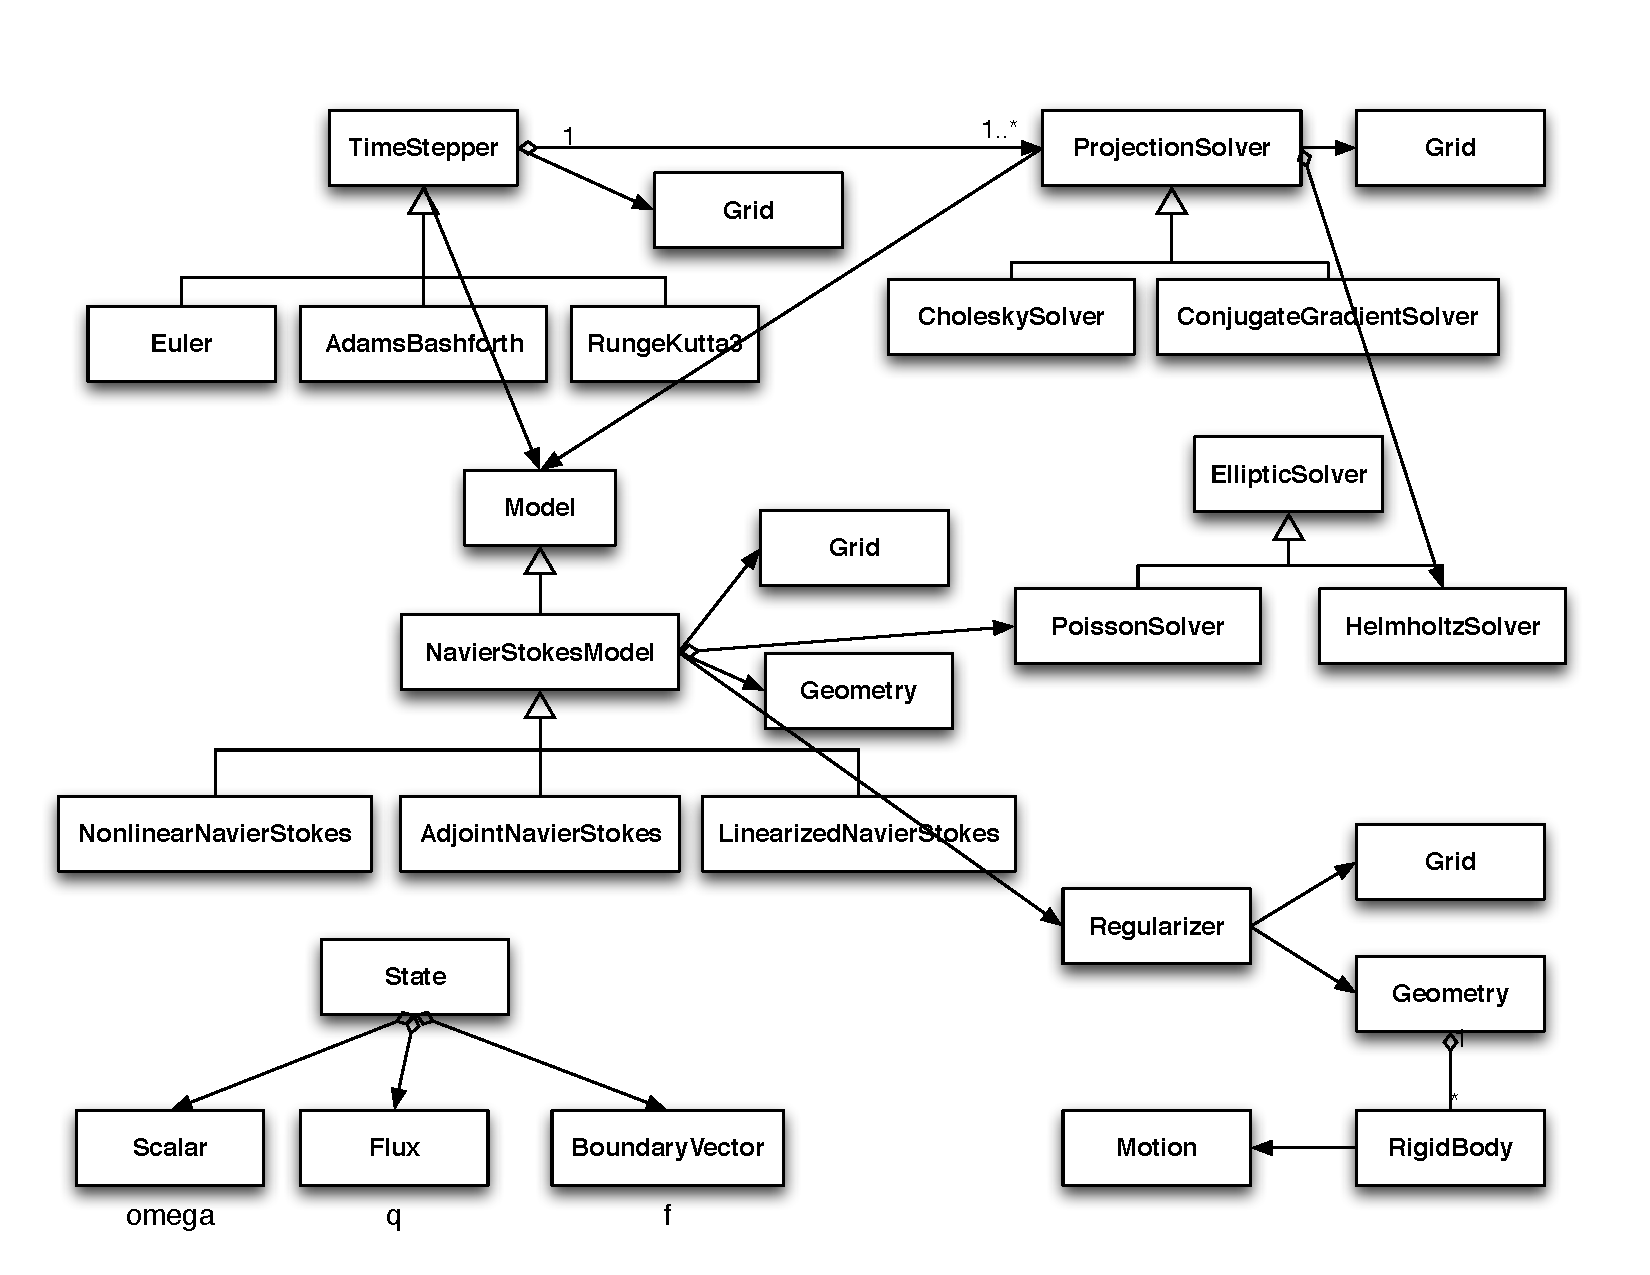
\includegraphics[width=\linewidth]{IBPMDesign}
	\caption{Overview of the various classes and their interactions.}
	\label{fig:classes}
\end{figure}

An overview of the classes and their interactions is shown in Figure~\ref{fig:classes}.

\subsection{Data structures}
\label{sub:data_structures}
The main data structures consist of a \class{Grid} that specifies the grid characteristics, a \class{Geometry} that specifies the configuration of the bodies and the locations of their boundary points, and variables that take on values either on the grid (\class{Scalar}, \class{Flux}), or on the boundary points (\class{BoundaryVector}).

A \class{Grid} defines the number of grid points in $x$- and $y$-directions, as well as the physical dimensions, and the number of grids to be used in a multi-domain solver.

Two classes, \class{Scalar} and \class{Flux}, define variables that take on values on the grid.  In particular, a \class{Scalar} variable (such as vorticity and streamfunction) takes on a single value at each node in Figure~\ref{fig:grid}. A \class{Flux} is vector-valued: the $x$-component is defined as the flux through vertical edges in Figure~\ref{fig:grid} (blue arrows), while the $y$-component is defined as the flux through horizontal edges (red arrows).

A \class{Geometry} defines the configuration of the bodies and the locations of their boundary points.  In particular, a \class{Geometry} contains a number of \class{RigidBody} objects, each with an associated \class{Motion} that prescribes the motion of that body in time.

A \class{BoundaryVector} defines a vector-valued function that takes on values at the boundary points defined by a particular \class{Geometry}.  For instance, the $x$- and $y$-forces at the boundary points are described by a \class{BoundaryVector}, as are the velocities at the boundary points, in the case of a moving body.

Finally, a \class{State} consists of the complete flow state at any time.  In particular, a \class{State} has components
\begin{center}
	\begin{tabular}{ll}
		\verb|Scalar omega|     & vorticity at each node\\
		\verb|Flux q|           & $u$- and $v$-velocity flux through cell edges\\
		\verb|BoundaryVector f| & forces at each of the boundary points\\
		\verb|int timestep|     & current timestep\\
		\verb|double time|      & current time
	\end{tabular}
\end{center}

\subsection{Mapping between grids and boundary points}
\label{sub:regularizer}
Sometimes one needs to map functions defined on boundary points onto a grid, or vice-versa, restrict values from a grid onto boundary points.  In Section~\ref{sec:method}, these operators were denoted $E^T$ and $E$, respectively.  In this library, the class that implements these operations is called \class{Regularizer}, and the sole purpose of the \class{Regularizer} is to compute these mappings, for a particular \class{Grid} and \class{Geometry}.

\subsection{Models}
\label{sub:models}
Various different sets of equations may be solved by the library, and each is specified as a type of \class{Model}.  Here, a \class{Model} specifies a set of equations of the form
\begin{equation}
\begin{aligned}
    \frac{d\omega}{dt} + Bf &= \alpha L\omega + N(x)\\
    C\omega &= b,
\end{aligned}
\label{eq:model}
\end{equation}
where $\omega$ is a \class{Scalar}, $f$ and~$b$ are \class{BoundaryVector}s, $x$ is a \class{State}, $L$ is the Laplacian, and the scalar~$\alpha$ and operators $B$, $C$, and $N$ are specified by the \class{Model}.

A \class{NavierStokesModel} is a subclass of \class{Model} that defines some version of the Navier-Stokes equations, for a particular \class{Grid}, \class{Geometry}, Reynolds number, and base flow.  Each \class{NavierStokesModel} contains a \class{PoissonSolver} (see Section~\ref{sub:elliptic_solvers}), for computing the streamfunction~$\psi$ from the vorticity~$\omega$, using
\[
	\nabla^2 \psi = -\omega,
\]
from which the corresponding velocity fluxes $q$ can then be computed as $q = \operatorname{curl} \psi + U_b$, where $U_b$ is a base flow.  The \class{NavierStokesModel} is responsible for all of this.

\class{NavierStokesModel} is an abstract base class, and may not be instantiated.  Its subclasses may, however, be instantiated, and are described below.  Note that, according to the formulation in~\cite{AhuRow-08}, the only difference between the nonlinear, linearized, and adjoint models is in the nonlinear term.

\class{NonlinearNavierStokes} defines the nonlinear Navier-Stokes equations.

\class{LinearizedNavierStokes} defines the Navier-Stokes equations linearized about an equilibrium point (steady solution).

\class{AdjointNavierStokes} defines the adjoint of the Navier-Stokes equations linearized about an equilibrium point.

\class{LinearizedPeriodicNavierStokes} defines the Navier-Stokes equations linearized about a periodic orbit.

\subsection{Timesteppers}
\label{sub:timesteppers}

Different types of timesteppers are available as well, for advancing the \class{State} forward in time.  Each \class{Timestepper} is associated with a particular \class{Grid} and \class{Model}, and a specific timestep~$h$.

In particular, a \class{Timestepper} advances governing equations in the form
(\ref{eq:model}), where $\omega$ is a \class{Scalar}, $f$ is a \class{BoundaryVector}, and $x$ is a \class{State}.  Here, $L$ is the Laplacian, and the other operators are defined in the associated instance of \class{Model}.

The sole purpose of a \class{Timestepper} is to provide a method ({\tt advance}) to march a \class{State} object forward to the next timestep.  For each type of timestepper, the projection method~(\ref{eq:projection_alg}) is used to solve for the next timestep.  This projection method is handled by a separate class, \class{ProjectionSolver}, and each \class{Timestepper} contains one or more \class{ProjectionSolver} instances.

\class{Timestepper} is an abstract base class, so only its subclasses may be instantiated.  These subclasses are described below.  

The \class{Euler} timestepper uses the Crank-Nicolson scheme to discretize the linear terms, and explicit Euler for the nonlinear term.  The resulting equations have the form
	\begin{align}
		(1-\frac{\alpha h}{2}L)\omega^{n+1} + hBf &= (1 + \frac{\alpha h}{2}L)\omega^n + h N(x^n)\\
		C\omega^{n+1} &= b_{n+1}
	\end{align}
where $h$ is the timestep.  Here, in the notation of~(\ref{eq:constrained}),
\begin{align}
	\mathcal{A} &= 1-\frac{\alpha h}{2} L\\
	\mathcal{B} &= hB\\
	\mathcal{C} &= C\\
	a &= (1+\frac{\alpha h}{2}L)\omega^n + hN(x^n)\\
	b &= b_{n+1},
\end{align}
where quantities on the right-hand side are specified by the associated \class{Model}.


The \class{AdamsBashforth} timestepper uses Crank-Nicolson for linear terms, and second-order Adams Bashforth for the nonlinear terms.  The resulting equations have the form
	\begin{align}
		(1-\frac{\alpha h}{2}L)\omega^{n+1} + hBf &= (1 + \frac{\alpha h}{2}L)\omega^n + \frac{h}{2} \big(3N(x^n) - N(x^{n-1})\big)\\
		C\omega^{n+1} &= b_{n+1}
	\end{align}
where $h$ is the timestep.  Here, in the notation of~(\ref{eq:constrained}),
\begin{equation}
	a = (1+\frac{\alpha h}{2}L)\omega^n + \frac{h}{2}(3N(x^n) - N(x^{n-1})
\end{equation}
with other parameters the same as \class{Euler}.  Because this is a multi-step scheme, an \class{AdamsBashforth} instance remembers the previous state that it computed.  This previous state can also be specified, via the method {\tt setPreviousState}.


The \class{RungeKutta2} timestepper uses Crank-Nicolson for the linear terms, and a second-order Runge-Kutta scheme for the nonlinear terms.  In particular, this class uses the scheme given by Peyret, p.~148\cite{Peyret:2002} (for Peyret's parameters $\alpha=1$, $\beta=1/2$):
\begin{align}
	(1 - \frac{\alpha h}{2}L)x_1 + hBf_1 &= (1+\frac{\alpha h}{2}L)x^n + hN(x^n)\\
	Cx_1 &= b_{n+1}\\
	(1-\frac{\alpha h}{2}L)x^{n+1} + hBf^{n+1} &= (1 + \frac{\alpha h}{2}L)x^n + \frac{h}{2}\big(N(x^n) + N(x_1)\big)\\
	Cx^{n+1} &= b_{n+1}.
\end{align}
		
The \class{RungeKutta3} timestepper uses Crank-Nicolson for linear terms, and a 3rd-order Runge-Kutta scheme for nonlinear terms.  In particular, this class uses the scheme given by Peyret, p.~149\cite{Peyret:2002}:
\begin{align}
	Q_1 &= hN(x^n)\\
	(1-\frac{\alpha h}{6}L)x_1 + \frac{h}{3}Bf_1 &= (1+\frac{\alpha h}{6}L)x^n + \frac{1}{3}Q_1\\
	Cx_1 &= b_{n+1/3}\\
	Q_2 &= -\frac{5}{9} Q_1 + hN(x_1)\\
	(1-\frac{5\alpha h}{24}L)x_2 + \frac{5h}{12}Bf_2 &= (1+\frac{5\alpha h}{24}L)x_1 + \frac{15}{16}Q_2\\
	Cx_2 &= b_{n+3/4}\\
	Q_3 &= -\frac{153}{128} Q_2 + hN(x_2)\\
	(1-\frac{\alpha h}{8}L)x^{n+1} + \frac{h}{4}Bf^{n+1} &= (1+\frac{\alpha h}{8}L)x_2 + \frac{8}{15}Q_3\\
	Cx^{n+1} &= b_{n+1}.
\end{align}

\subsection{Projection solver}
\label{sub:projection_solver}
The \class{ProjectionSolver} class implements the projection algorithm~(\ref{eq:projection_alg}).  In particular, it solves a system of the form
\begin{align}
   (1 - \frac{\alpha\beta}{2}L )x + \beta B f &= a\\
   C x &= b,
\end{align}
where $\alpha$ and the operators $B$ and~$C$ are determined by an associated \class{Model} instance, and the parameter~$\beta$ is specified to the \class{ProjectionSolver} instance.

\class{ProjectionSolver} is an abstract base class, as different strategies may be employed to solve the middle equation of~(\ref{eq:projection_alg}), depending on whether the operator on the left-hand side is constant, or time-dependent (i.e. when the body is moving, so the operators $\mathcal{B},\mathcal{C}$ vary in time).

\class{CholeskySolver} solves the middle equation of~(\ref{eq:projection_alg}) directly, using a Cholesky factorization, that is performed once and stored.  The Cholesky factorization may be saved to a file and loaded in to save time at startup.  This solver is much more efficient when the bodies are stationary, but if the bodies are moving, the factorization would need to be performed at each timestep, and in this case an iterative solver is faster.

\class{ConjugateGradientSolver} solves the middle equation of~(\ref{eq:projection_alg}) iteratively, using a conjugate gradient method, which is iterated to a specified tolerance.

\subsection{Elliptic solvers}
\label{sub:elliptic_solvers}

Elliptic equations such as Poisson or Helmholtz equations need to be solved at several places, and these solutions are computed by an \class{EllipticSolver} instance.  In particular, the \class{EllipticSolver} implements the multiple-domain solution described in Section~\ref{sec:method}.  A related class, \class{EllipticSolver2d}, solves a corresponding equation on a single, uniform grid (using a sin transform), and each \class{EllipticSolver} instance contains a number of \class{EllipticSolver2d} instances, one for each level of grid.

\class{EllipticSolver} is an abstract base class, and only its subclasses may be instantiated.  These subclasses are discussed below.

\class{PoissonSolver} solves a Poisson equation of the form
\[
	Lu = f
\]
with zero Dirichlet boundary conditions on $u$, where $L$ is the Laplacian, and $f$ is given.  The solver does some initial setup (computing eigenvalues of~$L$ at each grid level), and then can be used many times for different values of~$f$.

\class{HelmholtzSolver} solves a Helmholtz equation of the form
\[
	(1+\alpha L)u = f
\]
with zero Dirichlet boundary conditions on~$u$, where $L$ is the Laplacian, $\alpha$ is specified once to the solver, and the solver can be used many times for different values of~$f$.

\bibliographystyle{abbrv}
%\bibliography{jabbrv,master}
\bibliography{references}


\end{document}
